\subsection{Random Integers:}

The third test will consist in evaluate the running time of the algorithms analyzing an array of disordered random positive and negative integers of size $2^{5}$. \hfill \break

\begin{figure}[H]
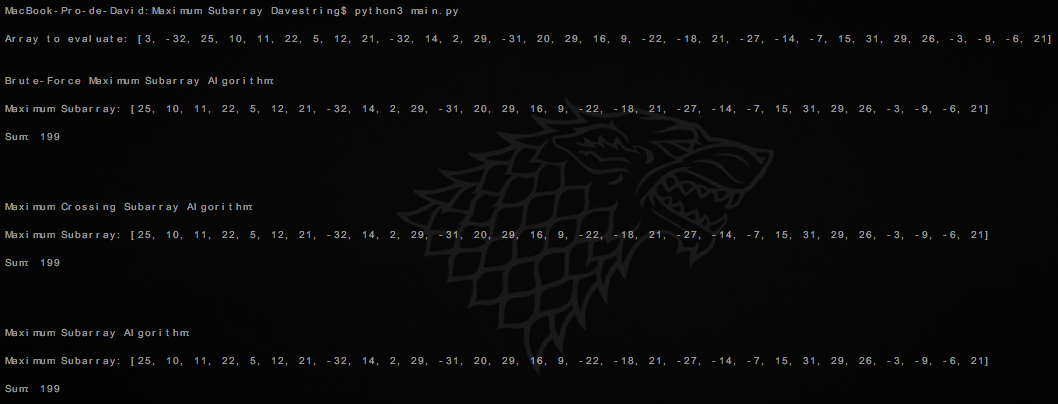
\includegraphics[width = 17cm, height = 10cm]{co3.png}
\centering \linebreak \linebreak Figure 4.2.0: Console output of the program.
\end{figure} \hfill 

\begin{figure}[H]
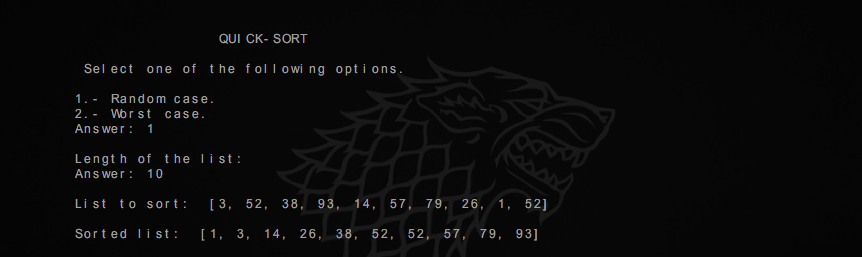
\includegraphics[width = 17cm, height = 10cm]{t3.png}
\centering \linebreak \linebreak Figure 4.2.1: Algorithms running time for an array of size $2^{5}$.
\end{figure} \hfill 

The following table shows the points of the plots where the first column it's the {\itshape Size} of the array, the second, third and fourth columns describes the computational time of {\itshape Brute-Force}, {\itshape Crossing} and {\itshape Recurrence} Maximum Subarray Algorithms respectively. \hfill \break

\begin{center} 
\begin{tabular}[.5cm]{ c c c c } 
\toprule 
\hspace{10pt} Size ( n ) \hspace{10pt} & \hspace{10pt} Brute-Force Time ( t ) \hspace{10pt} & \hspace{10pt} Crossing Time ( t ) \hspace{10pt} & \hspace{10pt} Recurrence Time ( t ) \\ 
\midrule 
0 & 7 & 8 & 0 \\ 
\cmidrule {1-4} 
1 & 17 & 13 & 2 \\ 
\cmidrule {1-4} 
2 & 25 & 18 & 29 \\ 
\cmidrule {1-4} 
3 & 39 & 23 & 61 \\ 
\cmidrule {1-4} 
4 & 59 & 28 & 93 \\ 
\cmidrule {1-4} 
5 & 81 & 33 & 130 \\ 
\cmidrule {1-4} 
6 & 97 & 34 & 163 \\ 
\cmidrule {1-4} 
7 & 123 & 39 & 200 \\ 
\cmidrule {1-4} 
8 & 147 & 44 & 237 \\ 
\cmidrule {1-4} 
9 & 169 & 49 & 279 \\ 
\cmidrule {1-4} 
10 & 193 & 52 & 315 \\ 
\cmidrule {1-4} 
11 & 219 & 55 & 355 \\ 
\cmidrule {1-4} 
12 & 247 & 58 & 395 \\ 
\cmidrule {1-4} 
13 & 281 & 63 & 435 \\ 
\cmidrule {1-4} 
14 & 313 & 66 & 471 \\ 
\cmidrule {1-4} 
15 & 347 & 69 & 509 \\ 
\cmidrule {1-4} 
16 & 387 & 74 & 551 \\ 
\cmidrule {1-4} 
17 & 429 & 79 & 598 \\ 
\cmidrule {1-4} 
18 & 477 & 90 & 653 \\ 
\cmidrule {1-4} 
19 & 519 & 93 & 690 \\ 
\cmidrule {1-4} 
20 & 563 & 96 & 723 \\ 
\cmidrule {1-4} 
21 & 609 & 99 & 770 \\ 
\cmidrule {1-4} 
22 & 657 & 98 & 807 \\ 
\cmidrule {1-4} 
23 & 707 & 101 & 842 \\ 
\cmidrule {1-4} 
24 & 759 & 104 & 889 \\ 
\cmidrule {1-4} 
25 & 813 & 107 & 930 \\ 
\cmidrule {1-4} 
26 & 869 & 114 & 981 \\ 
\cmidrule {1-4} 
27 & 931 & 119 & 1022 \\ 
\cmidrule {1-4} 
28 & 991 & 124 & 1069 \\ 
\cmidrule {1-4} 
29 & 1053 & 127 & 1106 \\ 
\cmidrule {1-4} 
30 & 1117 & 124 & 1141 \\ 
\cmidrule {1-4} 
31 & 1183 & 127 & 1180 \\ 
\cmidrule {1-4} 
32 & 1255 & 132 & 1227 \\ 
\bottomrule 
\linebreak 
\end{tabular} 
\linebreak \linebreak Table 2: Plot points of Figure 4.2.1.
\end{center} \hfill 

\pagebreak

The fourth test will consist in evaluate the running time of the algorithms analyzing an array of disordered random positive and negative integers of size $2^{4}$. \hfill \break

\begin{figure}[H]
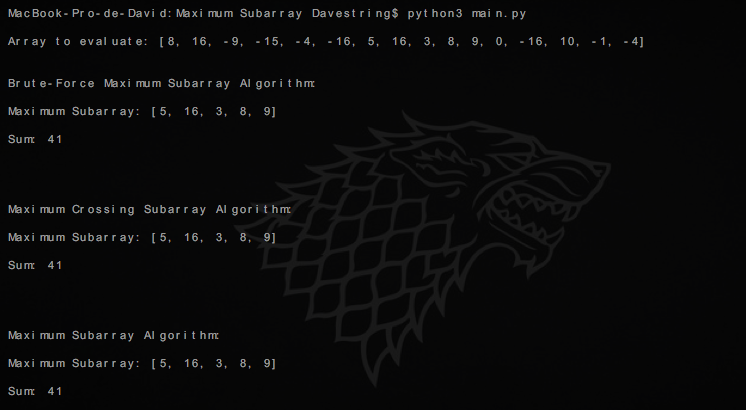
\includegraphics[width = 17cm, height = 10cm]{co4.png}
\centering \linebreak \linebreak Figure 4.2.2: Console output of the program.
\end{figure} \hfill 

\begin{figure}[H]
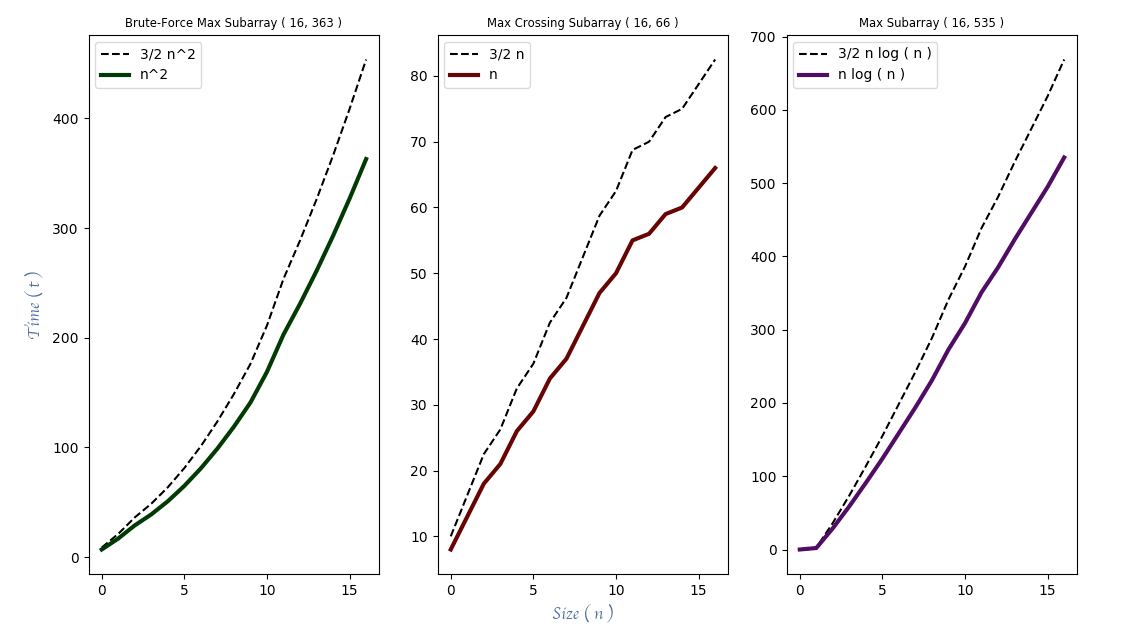
\includegraphics[width = 17cm, height = 10cm]{t4.png}
\centering \linebreak \linebreak Figure 4.2.3: Algorithms running time for an array of size $2^{4}$.
\end{figure} \hfill 

The following table shows the points of the plots where the first column it's the {\itshape Size} of the array, the second, third and fourth columns describes the computational time of {\itshape Brute-Force}, {\itshape Crossing} and {\itshape Recurrence} Maximum Subarray Algorithms respectively. \hfill \break

\begin{center} 
\begin{tabular}[.5cm]{ c c c c } 
\toprule 
\hspace{10pt} Size ( n ) \hspace{10pt} & \hspace{10pt} Brute-Force Time ( t ) \hspace{10pt} & \hspace{10pt} Crossing Time ( t ) \hspace{10pt} & \hspace{10pt} Recurrence Time ( t ) \\ 
\midrule 
0 & 7 & 8 & 0 \\ 
\cmidrule {1-4} 
1 & 17 & 13 & 2 \\ 
\cmidrule {1-4} 
2 & 29 & 18 & 29 \\ 
\cmidrule {1-4} 
3 & 39 & 21 & 59 \\ 
\cmidrule {1-4} 
4 & 51 & 26 & 91 \\ 
\cmidrule {1-4} 
5 & 65 & 29 & 124 \\ 
\cmidrule {1-4} 
6 & 81 & 34 & 159 \\ 
\cmidrule {1-4} 
7 & 99 & 37 & 194 \\ 
\cmidrule {1-4} 
8 & 119 & 42 & 231 \\ 
\cmidrule {1-4} 
9 & 141 & 47 & 273 \\ 
\cmidrule {1-4} 
10 & 169 & 50 & 309 \\ 
\cmidrule {1-4} 
11 & 203 & 55 & 351 \\ 
\cmidrule {1-4} 
12 & 231 & 56 & 385 \\ 
\cmidrule {1-4} 
13 & 261 & 59 & 423 \\ 
\cmidrule {1-4} 
14 & 293 & 60 & 459 \\ 
\cmidrule {1-4} 
15 & 327 & 63 & 495 \\ 
\cmidrule {1-4} 
16 & 363 & 66 & 535 \\ 
\bottomrule 
\linebreak 
\end{tabular} 
\linebreak \linebreak Table 3: Plot points of Figure 4.2.3.
\end{center} \hfill 

\pagebreak